% =====================================================================
%  Chapitre 4 -- partie b : ROC, desequilibre, calibration
% =====================================================================

\begin{frame}{La courbe ROC}
\begin{columns}[t]
\begin{column}{0.46\textwidth}
\centering
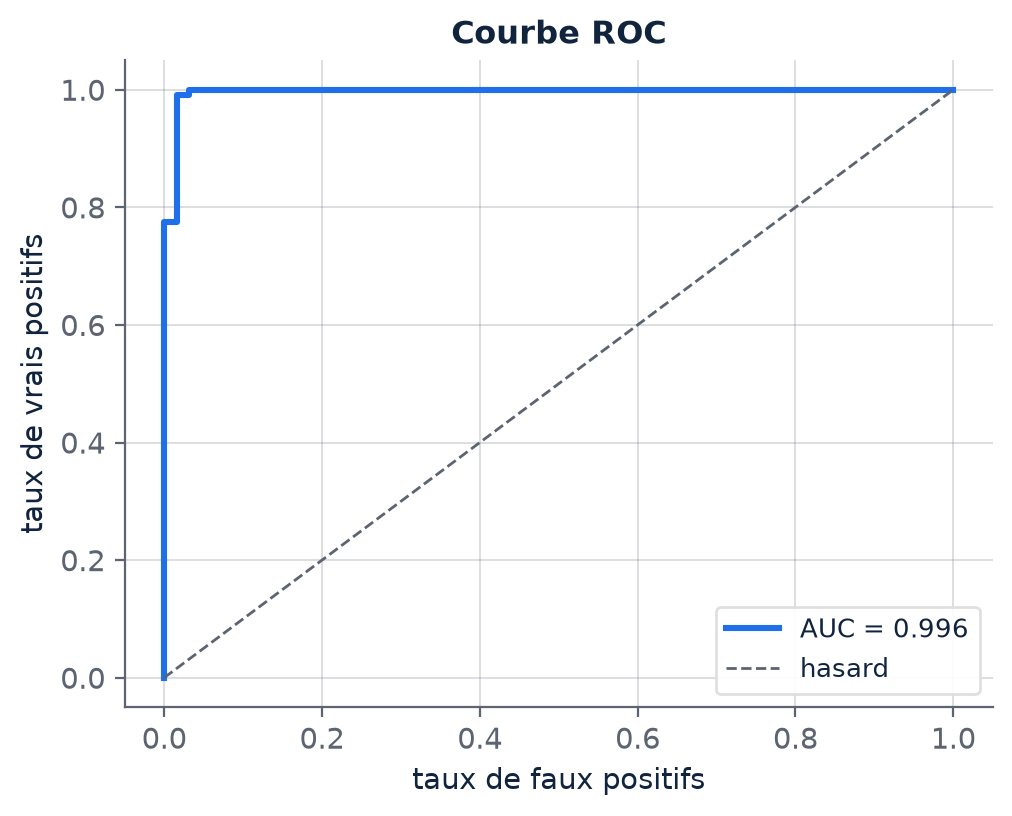
\includegraphics[height=0.32\textheight,keepaspectratio]{l05_roc.png}
\end{column}
\begin{column}{0.50\textwidth}
\begin{itemize}
  \item On fait varier le seuil de 1 à 0 et on trace (faux positifs, vrais
        positifs).
  \item Chaque point correspond à \textbf{un seuil}.
  \item Le coin supérieur gauche est le seuil idéal.
  \item Ici : AUC $=\mathbf{0{,}9963}$.
\end{itemize}
\begin{kbox}[Lecture de l'AUC]
Probabilité qu'un positif tiré au hasard soit mieux noté qu'un négatif tiré au
hasard. $0{,}5$ = hasard, $1$ = parfait.
\end{kbox}
\end{column}
\end{columns}
\end{frame}

\begin{frame}{Ce que l'AUC ne dit pas}
\begin{columns}[t]
\begin{column}{0.48\textwidth}
\begin{ebox}[Ce qu'elle résume bien]
La qualité du \textbf{classement} produit par le score, indépendamment du seuil
choisi.
\end{ebox}
\end{column}
\begin{column}{0.48\textwidth}
\begin{wbox}[Ce qu'elle cache]
Elle reste flatteuse sur des données très déséquilibrées : beaucoup de vrais
négatifs rendent le taux de faux positifs petit même avec de nombreuses alertes
fausses.
\end{wbox}
\end{column}
\end{columns}
\vspace{2mm}
\begin{kbox}[La bonne question]
« À quel seuil vais-je travailler, et que se passe-t-il \emph{à ce seuil} ? »
L'AUC seule ne répond pas.
\end{kbox}
\end{frame}

\begin{frame}{Comparer deux modèles}
\begin{columns}[t]
\begin{column}{0.50\textwidth}
\begin{itemize}
  \item Une courbe plus proche du coin supérieur gauche domine l'autre.
  \item Si les courbes se croisent, \textbf{aucun modèle n'est meilleur} :
        cela dépend du seuil et donc du coût.
  \item L'AUC résume, mais deux AUC égales peuvent cacher des courbes très
        différentes.
\end{itemize}
\end{column}
\begin{column}{0.46\textwidth}
\begin{wbox}[Le piège de l'AUC unique]
Un modèle excellent en zone de rappel élevé et un modèle excellent en zone de
précision élevée peuvent avoir la même AUC. Le choix dépend de l'usage.
\end{wbox}
\end{column}
\end{columns}
\vspace{2mm}
\begin{kbox}[La bonne pratique]
Comparer les deux modèles \textbf{au seuil d'exploitation}, avec le coût total
correspondant, et non seulement par un chiffre agrégé.
\end{kbox}
\end{frame}

\begin{frame}{Le coût total, en une formule}
\[
  C_{\text{total}}
  = C_{FP}\times FP \;+\; C_{FN}\times FN
  \;(+\; C_{VP}\times VP \text{ si le gain compte}).
\]
\begin{columns}[t]
\begin{column}{0.50\textwidth}
\begin{center}
\small
\begin{tabular}{@{}lrrr@{}}
\toprule
\textbf{Seuil} & $FP$ & $FN$ & \textbf{Coût} \\
\midrule
$0{,}5$ & $1$ & $2$ & $21$ \\
$0{,}3$ & $2$ & $0$ & $\mathbf{2}$ \\
$0{,}1$ & $6$ & $0$ & $6$ \\
\bottomrule
\end{tabular}
\end{center}
\end{column}
\begin{column}{0.46\textwidth}
Avec $C_{FP}=1$ et $C_{FN}=10$, le seuil $0{,}3$ gagne (coût $2$) : il détecte
tout en n'ajoutant qu'une fausse alerte. Descendre à $0{,}1$ \textbf{coûte plus
cher} sans rien détecter de plus.
\end{column}
\end{columns}
\vspace{1mm}
\begin{kbox}[La leçon]
Le bon seuil n'est pas celui qui maximise une métrique abstraite : c'est celui
qui minimise le coût réel, une fois ce coût écrit.
\end{kbox}
\end{frame}

\begin{frame}{Précision-rappel : l'outil du déséquilibre}
\begin{columns}[t]
\begin{column}{0.50\textwidth}
\centering
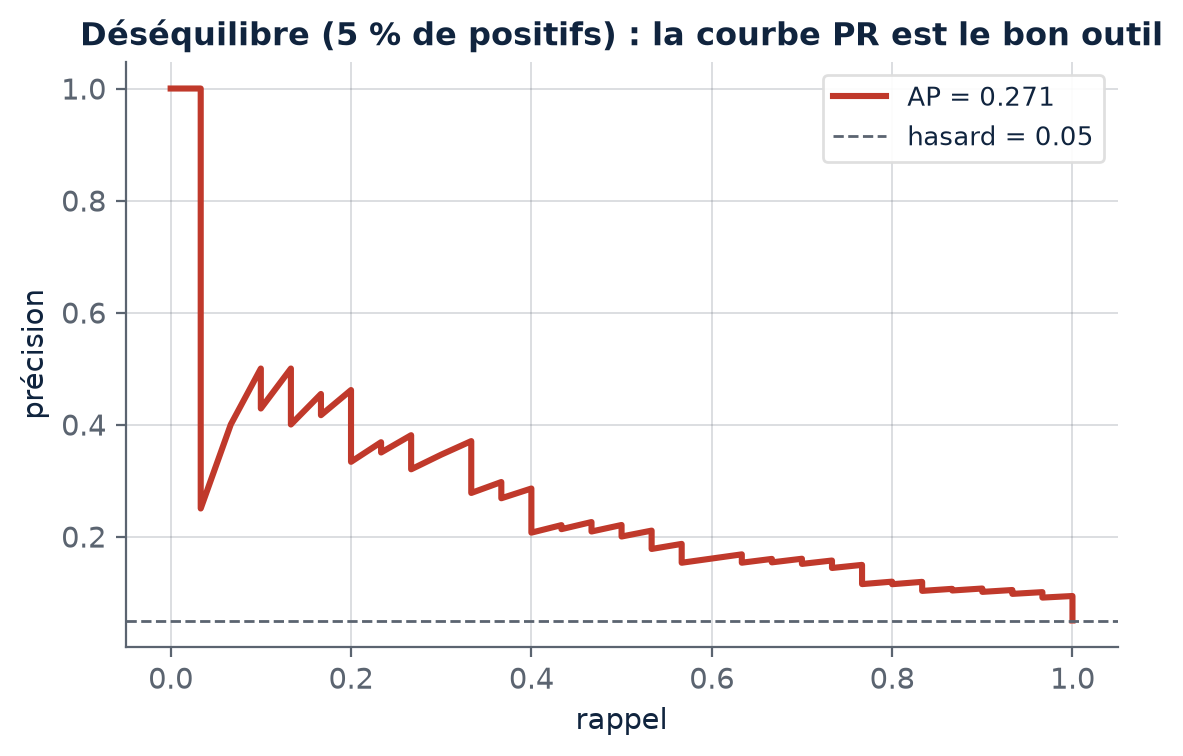
\includegraphics[height=0.31\textheight,keepaspectratio]{l06_pr.png}
\end{column}
\begin{column}{0.46\textwidth}
\begin{itemize}
  \item 5 \% de positifs seulement.
  \item Précision moyenne (AP) : $\mathbf{0{,}271}$.
  \item La ligne pointillée est le niveau du hasard : $0{,}05$.
\end{itemize}
\begin{kbox}[Pourquoi cette courbe]
Elle ne fait intervenir que les positifs et les alertes : les vrais négatifs,
qui sont légion, ne la gonflent pas.
\end{kbox}
\end{column}
\end{columns}
\end{frame}

\begin{frame}{L'exactitude menteuse}
\begin{columns}[t]
\begin{column}{0.52\textwidth}
\begin{center}
\small
\begin{tabular}{@{}lr@{}}
\toprule
\textbf{Modèle} & \textbf{Exactitude} \\
\midrule
Tout prédire « négatif » & $\mathbf{0{,}950}$ \\
Régression logistique & $\mathbf{0{,}950}$ \\
\bottomrule
\end{tabular}
\end{center}
\begin{wbox}[Le constat]
Le modèle n'apporte \textbf{rien} en exactitude, alors qu'il est le seul des
deux à détecter quelque chose.
\end{wbox}
\end{column}
\begin{column}{0.44\textwidth}
\begin{itemize}
  \item $F_1$ du modèle : $\mathbf{0{,}211}$.
  \item Rappel : $\mathbf{0{,}133}$ --- deux tiers des positifs manqués.
  \item AP : $0{,}271$, contre $0{,}05$ au hasard.
\end{itemize}
\begin{kbox}[La règle]
Sur données déséquilibrées, ne jamais annoncer l'exactitude seule.
\end{kbox}
\end{column}
\end{columns}
\end{frame}

\begin{frame}{Corriger le déséquilibre : la pondération}
\begin{columns}[t]
\begin{column}{0.52\textwidth}
\centering
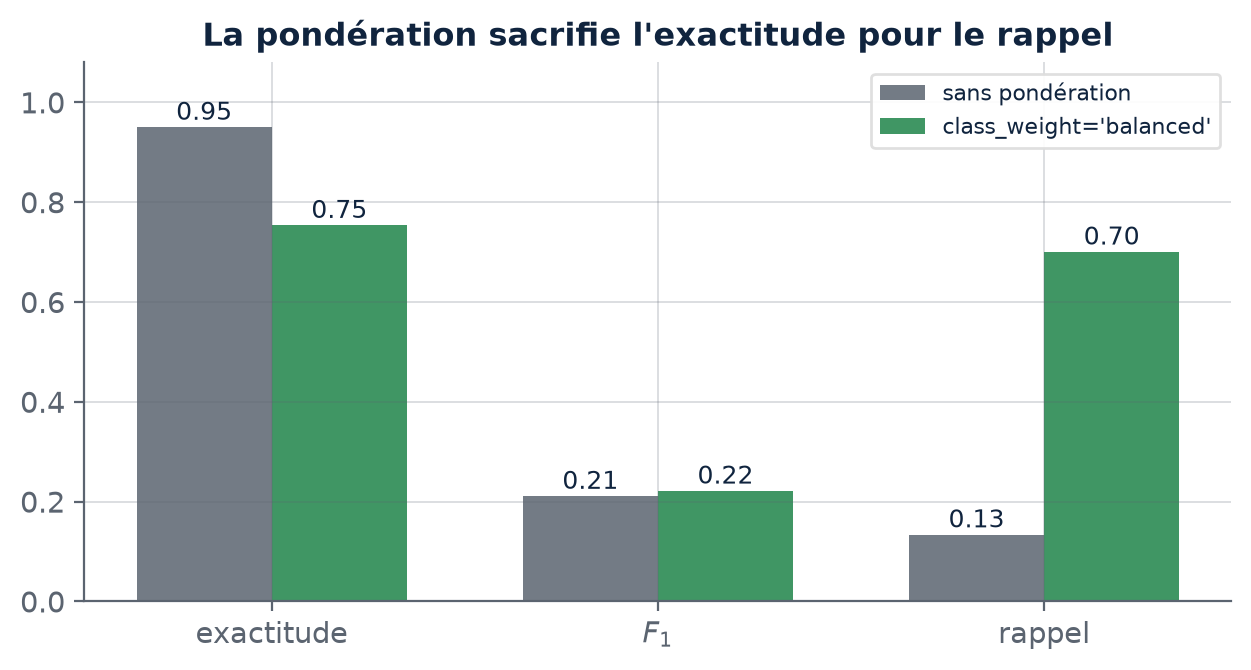
\includegraphics[height=0.30\textheight,keepaspectratio]{l07_ponderation.png}
\end{column}
\begin{column}{0.44\textwidth}
\begin{center}
\small
\begin{tabular}{@{}lrr@{}}
\toprule
 & \textbf{sans} & \textbf{avec} \\
\midrule
Exactitude & $0{,}950$ & $0{,}753$ \\
$F_1$ & $0{,}211$ & $0{,}221$ \\
Rappel & $0{,}133$ & $\mathbf{0{,}700}$ \\
\bottomrule
\end{tabular}
\end{center}
\begin{kbox}[Le compromis]
On perd 20 points d'exactitude pour gagner 57 points de rappel. C'est le bon
échange si un cas manqué coûte cher.
\end{kbox}
\end{column}
\end{columns}
\end{frame}

\begin{frame}{Les autres remèdes au déséquilibre}
\begin{center}
\small
\begin{tabular}{@{}p{0.20\textwidth}p{0.32\textwidth}p{0.38\textwidth}@{}}
\toprule
\textbf{Technique} & \textbf{Principe} & \textbf{Risque} \\
\midrule
Sous-échantillonnage & retirer des négatifs & perte d'information \\
Sur-échantillonnage & dupliquer des positifs & surapprentissage \\
SMOTE & interpoler de nouveaux positifs & positifs synthétiques irréalistes \\
Pondération & coût plus élevé pour la classe rare & à régler \\
Seuil adapté & décider à $0{,}1$ au lieu de $0{,}5$ & suppose la calibration \\
\bottomrule
\end{tabular}
\end{center}
\vspace{2mm}
\begin{kbox}[Le plus simple d'abord]
La pondération ne crée aucune donnée et se règle par validation croisée. C'est
le premier geste à essayer.
\end{kbox}
\end{frame}

\begin{frame}{Les probabilités sont-elles crédibles ?}
\begin{columns}[t]
\begin{column}{0.46\textwidth}
\centering
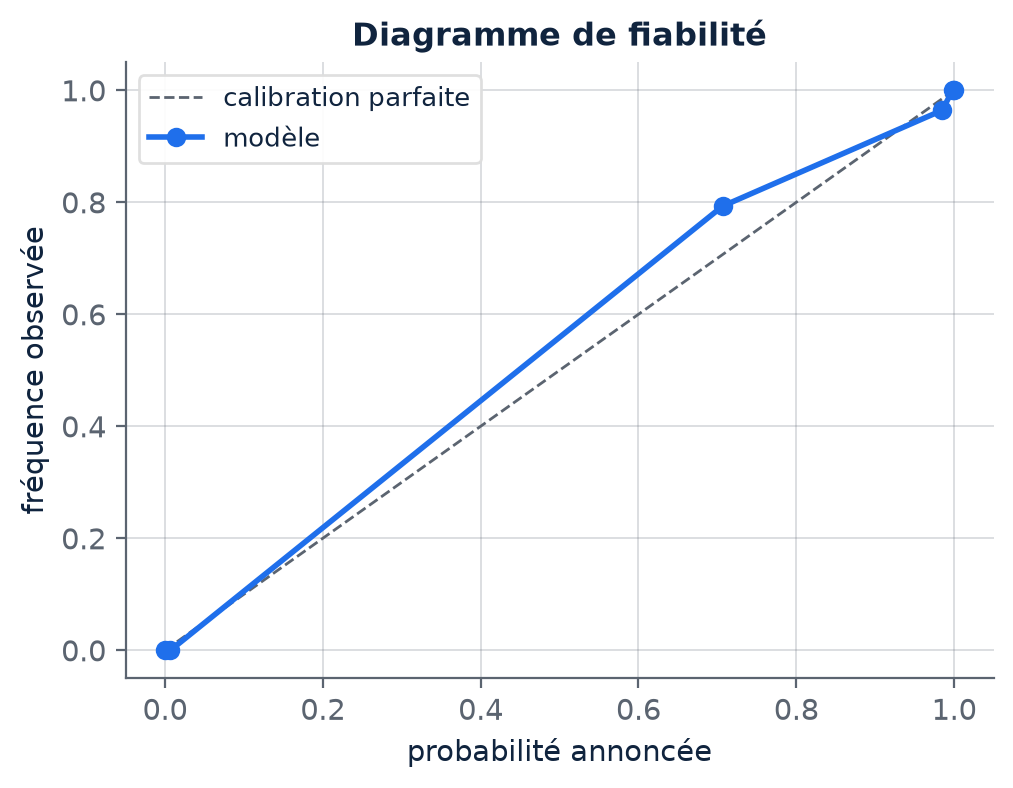
\includegraphics[height=0.31\textheight,keepaspectratio]{l08_calibration.png}
\end{column}
\begin{column}{0.50\textwidth}
\begin{itemize}
  \item Un modèle \textbf{calibré} : parmi les cas annoncés à 0,8, environ
        80 \% sont positifs.
  \item Ici, l'écart maximal observé est de $\mathbf{0{,}086}$.
  \item Au-dessus de la diagonale : le modèle sous-estime ; en dessous, il
        surestime.
\end{itemize}
\begin{kbox}[Comment corriger]
Régression isotonique ou \emph{Platt scaling}, ajustées sur un jeu de
validation séparé.
\end{kbox}
\end{column}
\end{columns}
\end{frame}

\begin{frame}{Ce qui casse la calibration}
\begin{columns}[t]
\begin{column}{0.48\textwidth}
\begin{itemize}
  \item Une forte régularisation écrase les probabilités vers le centre.
  \item Un rééchantillonnage change la prévalence : les probabilités ne
        correspondent plus au monde réel.
  \item Un modèle trop souple (arbre profond, forêt) donne des probabilités
        en escalier.
\end{itemize}
\end{column}
\begin{column}{0.48\textwidth}
\begin{wbox}[Conséquence pratique]
Après un SMOTE ou un sous-échantillonnage, il faut \textbf{recalibrer} avant
d'utiliser les probabilités dans un calcul de coût.
\end{wbox}
\begin{kbox}[Vérification]
Toujours tracer le diagramme de fiabilité avant d'annoncer « le modèle est
sûr à 90 \% ».
\end{kbox}
\end{column}
\end{columns}
\end{frame}

\begin{frame}{Validation croisée stratifiée}
\begin{columns}[t]
\begin{column}{0.48\textwidth}
\begin{wbox}[Le problème du $K$-Fold ordinaire]
Avec 5 \% de positifs, un pli peut n'en contenir aucun : la métrique devient
infinie ou indéfinie.
\end{wbox}
\end{column}
\begin{column}{0.48\textwidth}
\begin{solbox}[La solution]
\texttt{StratifiedKFold} conserve la proportion de classes dans chaque pli. Pour
des groupes (patients, écoles), \texttt{StratifiedGroupKFold}.
\end{solbox}
\end{column}
\end{columns}
\vspace{2mm}
\begin{kbox}[Et pour le temps]
Sur des séries temporelles, découpage chronologique obligatoire : jamais de
mélange aléatoire.
\end{kbox}
\end{frame}

\begin{frame}{Une métrique a une incertitude}
\begin{columns}[t]
\begin{column}{0.50\textwidth}
Avec 120 positifs et un rappel de 0,80, l'intervalle de confiance à 95 \%
vaut environ :
\[
  0{,}80 \pm 1{,}96\sqrt{\frac{0{,}8\times0{,}2}{120}}
  \;\approx\;[0{,}73\,;\,0{,}87].
\]
Deux modèles à 0,80 et 0,83 ne sont donc pas distinguables.
\end{column}
\begin{column}{0.46\textwidth}
\begin{kbox}[Le bootstrap]
Rééchantillonner les prédictions 1\,000 fois et lire les quantiles : valable
pour toute métrique, y compris le $F_1$ et l'AUC.
\end{kbox}
\begin{wbox}[Le piège]
Annoncer « 0,9874 » sans intervalle donne une fausse impression de précision.
\end{wbox}
\end{column}
\end{columns}
\end{frame}

\begin{frame}{Activité 2 --- déséquilibre (10 min)}
\begin{abox}[Détection de fraude]
1 transaction frauduleuse sur 200. Le modèle A a une exactitude de 0,995 et un
rappel de 0,02. Le modèle B a une exactitude de 0,94 et un rappel de 0,71.
\begin{enumerate}
  \item Lequel est le plus utile ? Pourquoi ?
  \item Que vaut l'exactitude d'un modèle qui ne détecte jamais rien ?
  \item Quelle métrique annoncer au comité de direction ?
\end{enumerate}
\end{abox}
\vspace{1mm}
\begin{solbox}[Réponses]
\textbf{1.} B : A rate 98 \% des fraudes. \textbf{2.} $199/200=0{,}995$ :
A ne fait pas mieux qu'un modèle vide. \textbf{3.} Rappel et précision (ou
coût total), accompagnés du nombre de fraudes détectées.
\end{solbox}
\end{frame}

\begin{frame}{Quiz 2 --- évaluation}
\begin{columns}[t]
\begin{column}{0.49\textwidth}
\begin{qbox}[Question 1]
Une AUC de 0,95 garantit :
\begin{itemize}
  \item[(a)] un bon rappel au seuil choisi
  \item[(b)] un bon classement global
  \item[(c)] des probabilités calibrées
\end{itemize}
\end{qbox}
\begin{qbox}[Question 2]
Sur 1 \% de positifs, la bonne courbe est :
\begin{itemize}
  \item[(a)] ROC \quad (b) précision-rappel
  \item[(c)] les deux, indifféremment
\end{itemize}
\end{qbox}
\end{column}
\begin{column}{0.49\textwidth}
\begin{qbox}[Question 3]
Après un SMOTE, il faut :
\begin{itemize}
  \item[(a)] recalibrer les probabilités
  \item[(b)] rien changer
  \item[(c)] augmenter le seuil
\end{itemize}
\end{qbox}
\begin{solbox}[Réponses]
\textbf{1.} (b) seulement. \quad \textbf{2.} (b). \quad \textbf{3.} (a).
\end{solbox}
\end{column}
\end{columns}
\end{frame}
